% ===============================================================
\chapter{Fregean Senses and Substitutivity}
% ===============================================================

\section{Senses}

\begin{definition}[Senses/meaning]
Whatever determines semantic value in Frege's Referential Theory of Meaning.
\end{definition}

Properties of senses:
\begin{enumerate}[label=\textbf{Property \arabic*:},leftmargin=*,align=left]
  \item They determine semantic value.
  \item They are compositional. Sense is a homomorphism across grammatical operations.
  \item They are abstract. They exist outside space and time.
  \item When a sentence is uttered, we grasp or interact with its sense.
\end{enumerate}

\section{The Fregean triangle}

\begin{minipage}{\linewidth}
\begin{center}
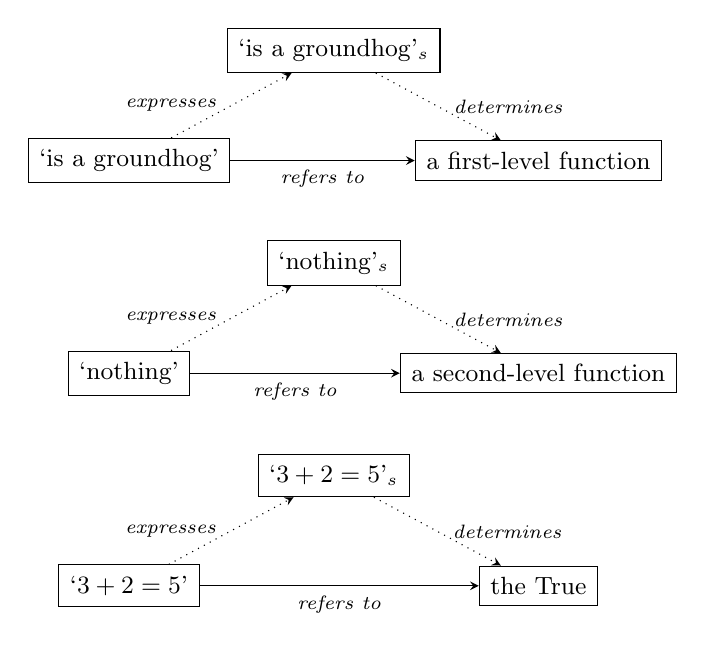
\begin{tikzpicture}[
    box/.style={draw, inner sep=4pt, font=\small},
    lab/.style={font=\scriptsize\itshape},
    >=stealth]
  \foreach \y/\expr/\val [count=\i] in
    {0/{`is a groundhog'}/{a first-level function},
     -2.7/{`nothing'}/{a second-level function},
     -5.4/{`$3+2=5$'}/{the True}} {
    \node[box] (s\i) at (0,\y) {\expr$_s$};
    \node[box] (e\i) at (-2.6,\y-1.4) {\expr};
    \node[box] (v\i) at (2.6,\y-1.4) {\val};
    \draw[->,dotted] (e\i) -- node[lab,left=2pt] {expresses} (s\i);
    \draw[->,dotted] (s\i) -- node[lab,right=2pt] {determines} (v\i);
    \draw[->] (e\i) -- node[lab,below] {refers to} (v\i);
  }
\end{tikzpicture}
\end{center}

\begin{enumerate}
  \item an expression \emph{expresses} its sense;
  \item a sense \emph{determines} a semantic value;
  \item an expression \emph{refers} to a semantic value determined by its sense.
\end{enumerate}
\end{minipage}

\begin{definition}
The sense of a sentence is a \emph{thought}.
\end{definition}

\section{Frege's antipsychologism}

\subsection*{The problem of communicative success}

Suppose meanings were mental entities, e.g.\ ideas or concepts. Since different people have different ideas or concepts, my meaning of `dog' might differ from your meaning of `dog'. But understanding a sentence requires understanding the meanings of the words comprising it, and successful communication requires mutual understanding. Thus, successful communication wouldn't be possible if you understand something different from `Fido is a dog' than I do. But successful communication is possible.

This implies that senses are not mental entities, and Frege therefore takes an antipsychologist view.

\section{The telescope analogy}

Suppose you and I both view Venus through a telescope. A single object---Venus---is projected on the lens of the telescope in both cases, but the same image is projected onto different retinas. Thus, you and I can see the same independently existing object despite processing the image of that object through different physiological means.

\begin{slide}
\begin{enumerate}
  \item \emph{The telescope: senses as objective}
  \begin{itemize}
    \item Venus :: the referent/semantic value of `Venus'
    \item image on the lens :: the objective sense/meaning of `Venus'
    \item image on the retina :: our subjective grasp of this sense
  \end{itemize}
  \item \emph{The microscope: logic as a guide to reality}
  \begin{itemize}
    \item image on the lens :: reality
    \item the microscope :: a logically perfect language
    \item the eye :: natural language
  \end{itemize}
\end{enumerate}
\end{slide}

\subsection{Solving the problem of cognitive significance}

\begin{itemize}
  \item Frege refers to senses as \emph{modes of presentation}.
  \item Given that senses are inherently distinct as modes of presentation, if there are two different senses, there are two different meanings despite the same referent. Senses are compositional, which means they express different thoughts. We know that thoughts are the sense of a sentence and therefore what we grasp, and then understand. This implies that what we grasp from a sentence with different senses is neither trivial nor uninformative.
\end{itemize}

\subsection{Solving the problem of empty names}

\begin{itemize}
  \item Sentences all have thoughts and therefore have sense.
  \item Compositionality implies that all expressions in the sentence also have senses.
  \item A sense does not require that a referent exists, according to Frege's RTM.
  \item This implies that all sentences can be meaningful.
\end{itemize}

\subsection{Solving the problem of Substitution Salva Veritate}

Substitution fails within indirect vs direct quotation and propositional attitude verbs. We distinguish between customary sense and indirect referent:

\begin{definition}\leavevmode
\begin{itemize}
  \item \emph{Customary sense}: the sense/\allowbreak referent of an expression outside the propositional attitude/\allowbreak quotation.
  \item \emph{Indirect referent}: the sense/\allowbreak referent of an expression inside the propositional attitude/\allowbreak quotation.
\end{itemize}
\end{definition}

Frege's solution is that \emph{the indirect referent of an expression is its customary sense}.

What does that mean? Inside a propositional attitude context, an expression refers to what is ordinarily its sense.

Given that the senses in an SSV sentence are not the same, they do not refer to the same thing, and by compositionality the sentences can differ in truth value.
